% Copyright (C) 2015 Glen Newton
% Author: Glen Newton
%  Licensed under a Creative Commons Attribution-NonCommercial-ShareAlike 4.0 International License

\documentclass{article}

\usepackage{tikz}
\usetikzlibrary{shapes.geometric,arrows,positioning,decorations.markings}

%\usepackage{helvet}

\renewcommand{\familydefault}{\sfdefault}

\pagestyle{empty}

\tikzstyle{vecArrow} = [thick, decoration={markings,mark=at position
   1 with {\arrow[semithick]{open triangle 60}}},
   double distance=4pt, shorten >= 4.5pt,
   preaction = {decorate},
   postaction = {draw,line width=4pt, white,shorten >= 4.5pt}]
\tikzstyle{innerWhite} = [semithick, white,line width=4pt, shorten >= 4.5pt]

\begin{document}
\hspace*{-4cm}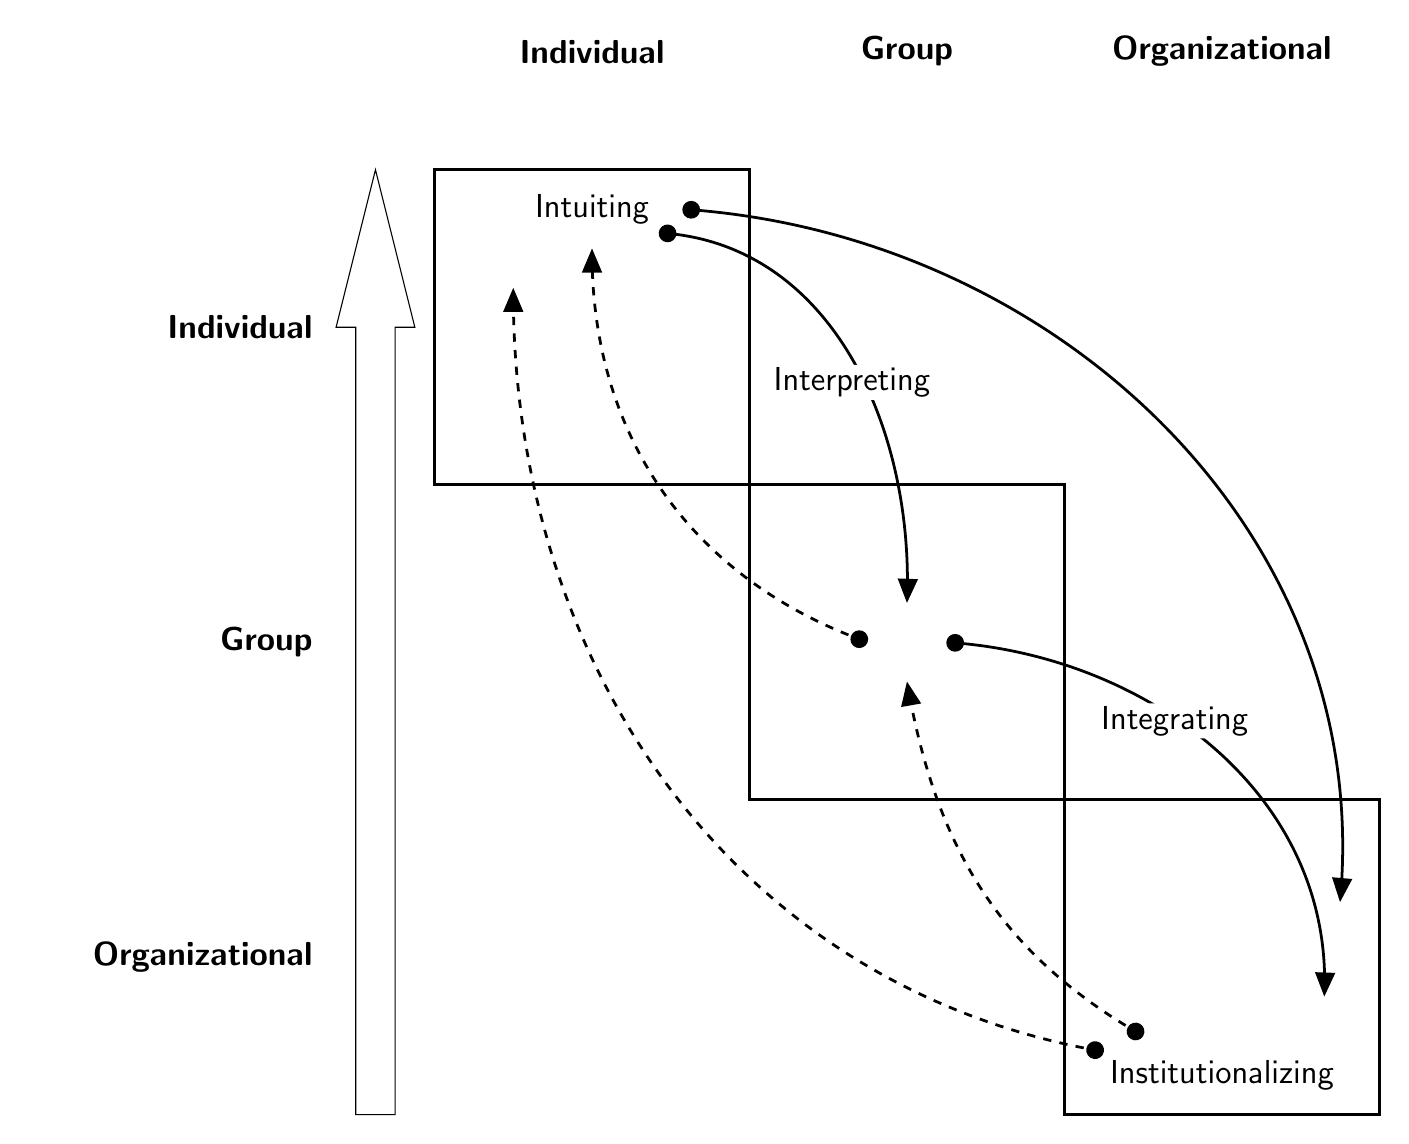
\begin{tikzpicture}
  \tikzset{>=triangle 45}



%%%%%%%%%%%%%%%%%%%%%%%%%%
  \node[draw,rectangle,minimum width=4cm,minimum height=4cm,inner sep=0pt,outer sep=0pt,line width=1pt] at (2,2) (A1) {};
  \node (NIntuiting) at ([yshift=15mm]A1.center) {\large Intuiting};

  %\draw[step=1cm,gray,very thin] (0,-8) grid (14,4);

%%%%%%%%%%%%%%%%%%%%%%%%%%
\node[draw,rectangle,minimum width=4cm,minimum height=4cm,inner sep=0pt,outer sep=0pt,line width=1pt] at (6,-2) (A2) {};

%%%%%%%%%%%%%%%%%%%%%%%%%%
\node[draw,rectangle,minimum width=4cm,minimum height=4cm,inner sep=0pt,outer sep=0pt,line width=1pt] at (10,-6) (A3) {};

%%%

%DOWN

\draw [*->,line width=1pt] ([yshift=-3mm]NIntuiting.east) to [out=-4,in=88] ([yshift=5mm]A2.center);
\draw [*->,line width=1pt] ([xshift=3mm]NIntuiting.east) to [out=-4,in=85] ([yshift=7mm,xshift=15mm]A3.center);
\draw [*->,line width=1pt] ([xshift=5mm]A2.center) to [out=-4,in=88] ([yshift=-5mm,xshift=13mm]A3.center);

% UP
\draw [*->,line width=1pt, dashed] ([xshift=-15mm,yshift=-12mm]A3.center) to [out=170,in=270] ([yshift=5mm,xshift=-10mm]A1.center);
\draw [*->,line width=1pt, dashed] ([xshift=-10mm,yshift=-10mm]A3.center) to [out=150,in=280] ([yshift=-5mm]A2.center);
\draw [*->,line width=1pt, dashed] ([xshift=-5mm]A2.center) to [out=160,in=270] ([yshift=10mm]A1.center);



\node (NIntegrating)[fill=white,rounded corners=2pt,inner sep=1pt] at ([xshift=14mm,yshift=-10mm]A2.east) {\large Integrating};
\node (NInstitutionalizing) at ([yshift=-15mm]A3.center) {\large Institutionalizing};
\node (NInterpreting)[fill=white,rounded corners=2pt,inner sep=1pt](NInterpreting) at ([xshift=13mm,yshift=-7mm]A1.east) {\large Interpreting};
%%%%%%%%%%%%%%%
%%%%%%%%%%%%%%%%%%



%TOP
\node (TopIndividual) at ([yshift=35mm]A1.center) {\large \bf Individual};
\node (TopGroup) at ([yshift=75mm]A2.center) {\large \bf Group};
\node (TopOrganizational) at ([yshift=115mm]A3.center) {\large \bf Organizational};

%SIDE
\node (SideIndividual)[text width=3.5cm,align=right] at ([xshift=-53mm]A1.center) {\large \bf \hfill Individual};
\node (SideGroup)[text width=3.5cm,align=right] at ([xshift=-93mm]A2.center) {\large \bf \hfill Group};
\node (SideOrganizational)[text width=3.5cm,align=right] at ([xshift=-133mm]A3.center) {\large \bf\hfill Organizational};

\draw   (-1,-8)--(-.50,-8)--(-.50,2)--(-.25,2)--(-.75,4)--(-1.25,2)--(-1,2)--cycle;




\end{tikzpicture}
\end{document}
